\documentclass{article}

\usepackage{swami}

\TL{}
\TM{Marvin Machine Specification}
\TR{}

\begin{document}
\noindent Marvin is a hypothetical computer with sixteen 32-bit registers and 16K 32-bit words of main memory (aka RAM). In addition to the sixteen registers, Marvin has a program counter \code{pc} and an instruction register \code{ir}. 

\bigskip

\noindent \textbf{Registers}: Marvin specifies the following conventions for its sixteen registers:
\begin{itemize}
\item \code{r0} -- \code{r2} (\code{a0} -- \code{a2}) are argument registers.
\item \code{r3} -- \code{r10} are general purpose registers.
\item \code{r11} (\code{ra}) is reserved to store the return address of the calling subroutine (aka function).
\item \code{r12} (\code{rv}) is reserved to store the return value of a subroutine.
\item \code{r13} (\code{fp}), called the frame pointer is reserved to store the base address of the most recent frame on the stack. It is initialized to 65,535 when the computer boots.
\item \code{r14} (\code{sp}), called the stack pointer, is reserved to store the address of the top of the stack. It is initialized to 65,535 when the computer boots.
\item \code{r15} (\code{gp}), called the global pointer, is reserved for to store the address of the top of the heap. It is initialized to 8,192 when the computer boots.
\end{itemize}

\bigskip

\noindent \textbf{Main Memory}: Marvin's main memory is divided into a text segment, a stack segment, and a heap segment, as shown below:

\smallskip

\begin{center}
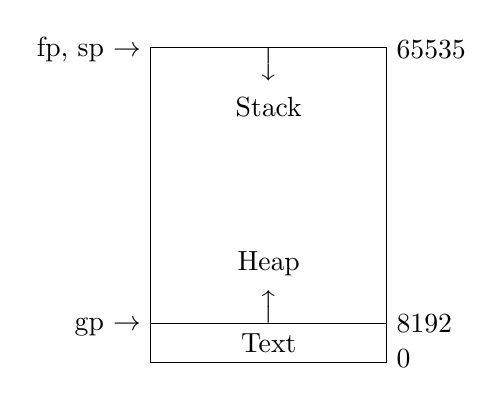
\begin{tikzpicture}

\draw (-1.5, 0) rectangle (1.5, 0.5) node[midway]{\code{Text}};
% \draw (-1.5, 0.5) rectangle (1.5, 2.25) node[midway]{\code{Heap}};
% \draw (-1.5, 2.25) rectangle (1.5, 4) node[midway]{\code{Stack}};
\node at (0, 1.25) {\code{Heap}};
\node at (0, 3.25) {\code{Stack}};
\draw (-1.5, 0.5) rectangle (1.5, 4);
\draw (1.5, 0.05) node[right]{\code{0}};
\draw (1.5, 0.5) node[right]{\code{8192}};
% \draw (1.5, 2.25) node[right]{\code{???}};
\draw (1.5, 3.98) node[right]{\code{65535}};
\draw (-1.5, 3.98) node[left]{\code{fp, sp} $\rightarrow$};
\draw (-1.5, 0.45) node[left]{\code{gp} $\rightarrow$};
\draw (0, 3.79) node{$\big\downarrow$};
\draw (0, 0.71) node{$\big\uparrow$};
\end{tikzpicture} 
\end{center}

\smallskip

\noindent The text segment extends from address 0 to address 8192. A Marvin program, which is a \code{.marv} file, is assembled and loaded into this segment starting at address 0.

\bigskip

\noindent The dynamic stack segment starts at address 65535 and grows downwards. This is where a subroutine's arguments, its local variables, and temporaries are stored.

\bigskip

\noindent The dynamic heap segment starts at address 8192 and grows upwards. This is where dynamically created objects are stored.
\bigskip

\noindent When a subroutine is called, a stack frame must be created for it on the stack, and it must be organized as shown below:

\smallskip

\begin{center}
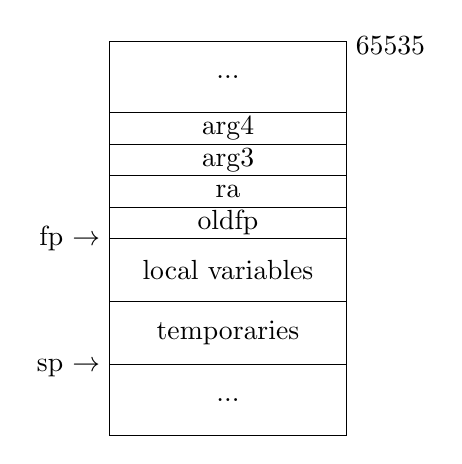
\begin{tikzpicture}
\draw (-1.5, 0) rectangle (1.5, 5);
\draw (1.5, 4.95) node[right]{\code{65535}};
\draw (-1.5, 5) rectangle (1.5, 4.1) node[midway]{\code{...}};
\draw (-1.5, 4.1) rectangle (1.5, 3.7) node[midway]{\code{arg4}};
\draw (-1.5, 3.7) rectangle (1.5, 3.3) node[midway]{\code{arg3}};
\draw (-1.5, 3.3) rectangle (1.5, 2.9) node[midway]{\code{ra}};
\draw (-1.5, 2.9) rectangle (1.5, 2.5) node[midway]{\code{oldfp}};
\draw (-1.5, 2.5) rectangle (1.5, 1.7) node[midway]{\code{local variables}};
\draw (-1.5, 1.7) rectangle (1.5, 0.9) node[midway]{\code{temporaries}};
\draw (-1.5, 0) rectangle (1.5, 0.9) node[midway]{\code{...}};
% \draw (1.5, 0.05) node[right]{\code{???}};
\draw (-1.5, 2.5) node[left]{\code{fp} $\rightarrow$};
\draw (-1.5, 0.85) node[left]{\code{sp} $\rightarrow$};
\end{tikzpicture} 
\end{center}

\newpage

\noindent \textbf{Instructions}: Marvin supports 53 instructions, each of which accepts between 0 and 3 arguments (aka inputs). Each category of instruction begins with a designated nibble (first four bits) followed by an operation specifier nibble.

\bigskip

\noindent System instructions (starting with the nibble \code{0000}):

\smallskip

% 12 instructions
\begin{boundedbox}
\begin{tabularx}{\columnwidth}{lll}
Opcode & 32-bit Machine Code & Description \brule 
\code{halt}          & \code{00000000 00000000 00000000 00000000} & stops the machine \grule
\code{readi rX}      & \code{00000001 00000000 00000000 0000XXXX} & sets \code{rX = N}, where \code{N} $\in [-2^{31}, 2^{31}-1]$ read from stdin \grule
\code{readf rX}      & \code{00000011 00000000 00000000 0000XXXX} & sets \code{rX = N}, where \code{N} is a float read from stdin \grule % TODO: wording
\code{readc rX}      & \code{00000101 00000000 00000000 0000XXXX} & sets \code{rX = N}, where \code{N} is a character read from stdin \grule
\code{writei rX}     & \code{00000010 00000000 00000000 0000XXXX} & writes integer \code{rX} to stdout \grule
\code{writef rX}     & \code{00000100 00000000 00000000 0000XXXX} & writes float \code{rX} to stdout \grule
\code{writec rX}     & \code{00000110 00000000 00000000 0000XXXX} & writes character \code{rX} to stdout \grule
\code{seed rX}       & \code{00000111 00000000 00000000 0000XXXX} & seeds the random number generator with \code{rX} \grule
\code{rand rX rY rZ} & \code{00001000 00000000 0000XXXX YYYYZZZZ} & sets \code{rX} to a random number in the range [\code{rY, rZ}] \grule 
\code{time rX}       & \code{00001001 00000000 00000000 0000XXXX} & sets \code{rX} to the time midnight \grule
% TODO: say something about the formatting
\code{date rX}       & \code{00001010 00000000 00000000 0000XXXX} & sets \code{rX} to the current date \grule
\code{nop}           & \code{00001111 00000000 00000000 00000000} & does nothing
\end{tabularx}
\end{boundedbox}

\bigskip

\noindent Arithmetic instructions (starting with the nibble \code{0001}):

\smallskip

% 11 instructions
\begin{boundedbox}
\begin{tabularx}{\columnwidth}{lll}
Opcode & 32-bit Machine Code & Description \brule 
\code{add rX rY rZ}  & \code{00010000 00000000 0000XXXX YYYYZZZZ} & sets \code{rX = rY + rZ} for integers \grule
\code{sub rX rY rZ}  & \code{00010001 00000000 0000XXXX YYYYZZZZ} & sets \code{rX = rY - rZ} for integers \grule
\code{mul rX rY rZ}  & \code{00010010 00000000 0000XXXX YYYYZZZZ} & sets \code{rX = rY * rZ} for integers \grule
\code{div rX rY rZ}  & \code{00010011 00000000 0000XXXX YYYYZZZZ} & sets \code{rX = rY // rZ} for integers \grule
\code{mod rX rY rZ}  & \code{00010100 00000000 0000XXXX YYYYZZZZ} & sets \code{rX = rY \% rZ} for integers \grule
\code{neg rX rY}     & \code{00010101 00000000 00000000 XXXXYYYY} & sets \code{rX = -rY} for integers \grule
\code{fadd rX rY rZ} & \code{00010110 00000000 0000XXXX YYYYZZZZ} & sets \code{rX = rY + rZ} for floating point numbers \grule
\code{fsub rX rY rZ} & \code{00010111 00000000 0000XXXX YYYYZZZZ} & sets \code{rX = rY - rZ} for floating point numbers \grule
\code{fmul rX rY rZ} & \code{00011000 00000000 0000XXXX YYYYZZZZ} & sets \code{rX = rY * rZ} for floating point numbers \grule
\code{fdiv rX rY rZ} & \code{00011001 00000000 0000XXXX YYYYZZZZ} & sets \code{rX = rY // rZ} for floating point numbers \grule
\code{fneg rX rY}    & \code{00011010 00000000 00000000 XXXXYYYY} & sets \code{rX = -rY} for floating point numbers
\end{tabularx}
\end{boundedbox}

\newpage

\noindent Bitwise instructions (starting with the nibble \code{0010}):

\smallskip

% 8 instructions
% TODO: change wording e.g. rX = rY XOR rZ
\begin{boundedbox}
\begin{tabularx}{\columnwidth}{lll}
Opcode & 32-bit Machine Code & Description \brule 
\code{and rX rY rZ} & \code{00100000 00000000 0000XXXX YYYYZZZZ} & bitwise ANDs \code{rY} by \code{rZ}, placing the result in \code{rX} \grule
\code{or rX rY rZ}  & \code{00100001 00000000 0000XXXX YYYYZZZZ} & bitwise ORs \code{rY} by \code{rZ}, placing the result in \code{rX} \grule
\code{xor rX rY rZ} & \code{00100010 00000000 0000XXXX YYYYZZZZ} & bitwise XORs \code{rY} by \code{rZ}, placing the result in \code{rX} \grule
\code{not rX rY rZ} & \code{00100011 00000000 0000XXXX YYYYZZZZ} & bitwise NOTs \code{rY} by \code{rZ}, placing the result in \code{rX} \grule
\code{lshl rX rY}   & \code{00100100 00000000 00000000 XXXXYYYY} & logical shifts \code{rY} \code{rZ} bits to the left \grule
\code{lshr rX rY}   & \code{00100101 00000000 00000000 XXXXYYYY} & logical shifts \code{rX} \code{rY} bits to the right \grule
\code{ashl rX rY}   & \code{00100110 00000000 00000000 XXXXYYYY} & arithmetic shifts integer \code{rX} \code{rY} bits to the left \grule
\code{ashr rX rY}   & \code{00100111 00000000 00000000 XXXXYYYY} & arithmetic shifts integer \code{rX} \code{rY} bits to the right
\end{tabularx}
\end{boundedbox}

\bigskip

\noindent Jump instructions (starting with the nibble \code{0011}):

\smallskip

% 11 instructions
\begin{boundedbox}
\begin{tabularx}{\columnwidth}{lll}
Opcode & 32-bit Machine Code & Description \brule 
\code{jumpn N}      & \code{00110000 00000000 NNNNNNNN NNNNNNNN} & jumps to instruction \code{N} \grule
\code{jumpr rX}     & \code{00110001 00000000 00000000 0000XXXX} & jumps to instruction \code{rX} \grule
\code{jeqzn rX N}   & \code{00110010 0000XXXX NNNNNNNN NNNNNNNN} & jumps to instruction \code{N} if \code{rX == 0} \grule
\code{jnezn rX N}   & \code{00110011 0000XXXX NNNNNNNN NNNNNNNN} & jumps to instruction \code{N} if \code{rX != 0} \grule
\code{jgen rX rY N} & \code{00110100 XXXXYYYY NNNNNNNN NNNNNNNN} & jumps to instruction \code{N} if \code{rX >= rY} \grule
\code{jlen rX rY N} & \code{00110101 XXXXYYYY NNNNNNNN NNNNNNNN} & jumps to instruction \code{N} if \code{rX <= rY} \grule
\code{jeqn rX rY N} & \code{00110110 XXXXYYYY NNNNNNNN NNNNNNNN} & jumps to instruction \code{N} if \code{rX == rY} \grule
\code{jnen rX rY N} & \code{00110111 XXXXYYYY NNNNNNNN NNNNNNNN} & jumps to instruction \code{N} if \code{rX != rY} \grule
\code{jgtn rX rY N} & \code{00111000 XXXXYYYY NNNNNNNN NNNNNNNN} & jumps to instruction \code{N} if \code{rX > rY} \grule
\code{jltn rX rY N} & \code{00111001 XXXXYYYY NNNNNNNN NNNNNNNN} & jumps to instruction \code{N} if \code{rX < rY} \grule
\code{calln rX N}   & \code{00111010 0000XXXX NNNNNNNN NNNNNNNN} & sets \code{rX = pc + 1} and jumps to instruction \code{N}
\end{tabularx}
\end{boundedbox}

\bigskip

\noindent Instructions for setting register data (starting with the nibble \code{0100}):

\smallskip

% 5 instructions
\begin{boundedbox}
\begin{tabularx}{\columnwidth}{lll}
Opcode & 32-bit Machine Code & Description \brule 
\code{seti rX N}  & \code{01000000 0000XXXX NNNNNNNN NNNNNNNN} & sets \code{rX = N}, where \code{N} $\in [-2^{15}, 2^{15}-1]$ \grule
\code{addi rX N}  & \code{01000001 0000XXXX NNNNNNNN NNNNNNNN} & sets \code{rX = rX + N}, where \code{N} $\in [-2^{15}, 2^{15}-1]$ \grule
\code{setf rX F}  & \code{01000010 0000XXXX FFFFFFFF FFFFFFFF} & sets \code{rX = F}, where \code{F} is a floating point number \grule
\code{addf rX F}  & \code{01000011 0000XXXX FFFFFFFF FFFFFFFF} & sets \code{rX = rX + F}, where \code{F} is a floating point number  \grule
\code{copy rX rY} & \code{01000100 00000000 00000000 XXXXYYYY} & sets \code{rX = rY}
\end{tabularx}
\end{boundedbox}

\newpage

\noindent Instructions for interacting with the stack (starting with the nibble \code{0101}):

\smallskip

% 6 instructions
\begin{boundedbox}
\begin{tabularx}{\columnwidth}{lll}
Opcode & 32-bit Machine Code & Description \brule 
% TODO: descriptions

% push/pop byte
\code{pushrb rX rY}    & \code{01010000 00000000 00000000 XXXXYYYY} & sets \code{mem[rY--] = rX} \grule
\code{poprb rX rY}     & \code{01010001 00000000 00000000 XXXXYYYY} & sets \code{rX = mem[++rY]} \grule
% push/pop short
\code{pushrs rX rY}    & \code{01010010 00000000 00000000 XXXXYYYY} & sets \code{mem[rY--] = rX} \grule
\code{poprs rX rY}     & \code{01010011 00000000 00000000 XXXXYYYY} & sets \code{rX = mem[++rY]} \grule
% push/pop word
\code{pushrw rX rY}    & \code{01010100 00000000 00000000 XXXXYYYY} & sets \code{mem[rY--] = rX} \grule
\code{poprw rX rY}     & \code{01010101 00000000 00000000 XXXXYYYY} & sets \code{rX = mem[++rY]}
\end{tabularx}
\end{boundedbox}

\noindent Instructions for interacting with memory (starting with the nibble \code{0110}):

\smallskip

% 12 instructions
\begin{boundedbox}
\begin{tabularx}{\columnwidth}{lll}
Opcode & 32-bit Machine Code & Description \brule 
% TODO: descriptions

% loads/stores for byte
\code{loadnb rX rY N}  & \code{01100000 XXXXYYYY NNNNNNNN NNNNNNNN} & sets \code{rX = mem[rY + N]}, where \code{N} $\in [-2^{15}, 2^{15}-1]$ \grule
\code{storenb rX rY N} & \code{01100001 XXXXYYYY NNNNNNNN NNNNNNNN} & sets \code{mem[rY + N] = rX}, where \code{N} $\in [-2^{15}, 2^{15}-1]$ \grule
\code{loadrb rX rY}    & \code{01100010 00000000 00000000 XXXXYYYY} & sets \code{rX = mem[rY]} \grule
\code{storerb rX rY}   & \code{01100011 00000000 00000000 XXXXYYYY} & sets \code{mem[rY] = rX} \grule
% loads/stores for short
\code{loadns rX rY N}  & \code{01100100 XXXXYYYY NNNNNNNN NNNNNNNN} & sets \code{rX = mem[rY + N]}, where \code{N} $\in [-2^{15}, 2^{15}-1]$ \grule
\code{storens rX rY N} & \code{01100101 XXXXYYYY NNNNNNNN NNNNNNNN} & sets \code{mem[rY + N] = rX}, where \code{N} $\in [-2^{15}, 2^{15}-1]$ \grule
\code{loadrs rX rY}    & \code{01100110 00000000 00000000 XXXXYYYY} & sets \code{rX = mem[rY]} \grule
\code{storers rX rY}   & \code{01100111 00000000 00000000 XXXXYYYY} & sets \code{mem[rY] = rX} \grule
% loads/stores for word
\code{loadnw rX rY N}  & \code{01101000 XXXXYYYY NNNNNNNN NNNNNNNN} & sets \code{rX = mem[rY + N]}, where \code{N} $\in [-2^{15}, 2^{15}-1]$ \grule
\code{storenw rX rY N} & \code{01101001 XXXXYYYY NNNNNNNN NNNNNNNN} & sets \code{mem[rY + N] = rX}, where \code{N} $\in [-2^{15}, 2^{15}-1]$ \grule
\code{loadrw rX rY}    & \code{01101010 00000000 00000000 XXXXYYYY} & sets \code{rX = mem[rY]} \grule
\code{storerw rX rY}   & \code{01101011 00000000 00000000 XXXXYYYY} & sets \code{mem[rY] = rX}
\end{tabularx}
\end{boundedbox}

\bigskip

\noindent \textbf{Marvin Emulator}: The Python program \code{marvin.py} serves as an emulator for the Marvin machine. Here is the usage syntax for the program:

\smallskip

\begin{window}[\tilde/workspace/marvin]
\begin{codeblock}[]{{}}
$ python3 marvin.py -h

usage: marvin [-h] [-v] [-d] filename

This program serves as an emulator for a register-based machine called Marvin (named 
after the paranoid android character, Marvin, from The Hitchhiker's Guide to the 
Galaxy by Douglas Adams). The design of the machine was inspired by that of the 
Harvey Mudd Miniature Machine (HMMM) developed at Harvey Mudd College. The program 
accepts a .marv file as input, assembles and simulates the instructions within, and 
prints any output to stdout. Any input to the .marv program is via stdin. If the 
optional -v argument is specified, the emulator prints the assembled instructions 
to stdout before simulating them.

positional arguments:
  filename       input .marv file

options:
  -h, --help     show this help message and exit
  -v, --verbose  enable verbose output
  -d, --debug    enable debug mode
$ _
\end{codeblock}
\end{window}

\bigskip

\noindent Here is a sample Marvin program called \code{Coundown.marv} that accepts $n$ (int) from standard input and writes to standard output a countdown from $n$ to 0.

\smallskip

\begin{window}[Countdown.marv]
\begin{codeblock}[]{{}}
# Accepts n (int) from standard input and writes a countdown from n to 0 to standard 
# output.

0    read     r0          # read n
1    set0     r1          # zero = 0
2    jltn     r0 r1 6     # if n < zero jump to 6
3    write    r0          # write n
4    addn     r0 -1       # n = n - 1
5    jumpn    2           # jump to 2
6    halt                 # halt the machine
\end{codeblock}
\end{window}

\bigskip

\noindent Here is the output from running \code{Countdown.marv} using \code{marvin.py}, which is an emulator for the Marvin machine.

\smallskip

\begin{window}[\tilde/workspace/marvin]
\begin{codeblock}[]{{}}
$ python3 marvin.py -v Countdown.marv
    0: 00000001 00000000 00000000 00000000                    0: read   r0  
    1: 00000100 00000000 00000000 00000001                    1: set0   r1  
    2: 00011000 00000001 00000000 00000110                    2: jltn   r0 r1 6
    3: 00000010 00000000 00000000 00000000                    3: write  r0  
    4: 00000111 00000000 10000000 00000001                    4: addn   r0 -1 
    5: 00001111 00000000 00000000 00000010                    5: jumpn  2  
    6: 00000000 00000000 00000000 00000000                    6: halt     

5
5
4
3
2
1
0
$ _
\end{codeblock}
\end{window}
\end{document}

